\section{Extra-galactic sources}\label{sec:Extragal}

We have so far only been concerned with properties of bursts from our own galaxy. This is the best source for bursts because of its proximity. A natural continuation is to consider EMRBs from other MBHs. \citet{Rubbo2006} suggested that LISA should be able to detect EMRBs originating from the Virgo cluster, although the detectable rate might only be $10^{-4}\units{yr^{-1}}$ per galaxy \citep{Hopman2007}. We wish to investigate this possibility using our more accurate waveforms.

\subsection{Detection with LISA}

Space-based detectors are most sensitive from extreme-mass-ratio signals originating from MBHs with masses $10^5$--$10^6 M_\odot$. Higher mass objects produce signals at too low frequencies. We considered several nearby MBHs that were likely candidates for detectable burst signals. Details are given in \tabref{MBHs}.
\begin{table}[htp]
%\begin{minipage}{\columnwidth}
 \centering
  \begin{tabular}{p{0.2\textwidth} D{.}{.}{3.2} D{.}{.}{2.5} p{0.45\textwidth}}
  \toprule
   Galaxy & \multicolumn{1}{c}{$M_\bullet/10^6 M_\odot$} & \multicolumn{1}{c}{$R/\mathrm{Mpc}$} & References \\
 \midrule
 Milky Way (GC) & 4.31 & 0.00833& \citet{Gillessen2009} \\
 M32 (NGC 221) & 2.5 & 0.770 & \citet{Verolme2002,Karachentsev2004} \\
 Andromeda (M31, NGC 224) & 140 & 0.770 &  \citet{Bender2005,Karachentsev2004} \\
 Circinus & 1.1 & 2.82 & \citet{Graham2008,Greenhill2003,Karachentsev2007} \\
 NGC 4945 & 1.4 & 3.82	& \citet{Greenhill1997,Karachentsev2007} \\
 Sculptor (NGC 253) & 10 & 3.5 & \citet{Graham2011,Rodriguez-Rico2006,Rekola2005} \\
 NGC 4395 & 0.36 & 4.0& \citet{Peterson2005,Thim2004} \\
 NGC 3368 & 7.3 & 10.1 & \citet{Graham2011,Nowak2010,Tonry2001} \\
 NGC 3489 & 5.8 & 11.7 & \citet{Graham2011,Nowak2010,Tonry2001} \\
\bottomrule
\end{tabular}
\caption{Sample of nearby MBHs that are candidates for producing detectable EMRBs.\label{tab:MBHs}}
%\end{minipage}
\end{table}
For each, we calculated SNRs at $\sim 10^4$ different periapse distances following the same method as in \secref{wave-ex}.

The SNR depends upon many parameters. For a given MBH, the most important parameter is the periapse radius $r\sub{p}$. As shown in \figref{SNR}, there is a good correlation between $\rho$ and $r\sub{p}$; other parameters only produce scatter about this. The form of the $\rho$--$r\sub{p}$ relation depends upon the noise curve. To compare SNRs between MBHs, we parametrize the detectability in terms of a characteristic frequency
\begin{equation}
f_\ast = \sqrt{\frac{GM_\bullet}{r\sub{p}^3}}.
\end{equation}
This allows comparison between different systems where the same periapse does not correspond to the same frequency, and thus the same point of the noise curve.

We also expect the SNR to scale with other quantities. We define a characteristic strain amplitude for a burst $h_0$; we expect $\rho \propto h_0$, where the proportionality is set by a frequency-dependent function that includes the effect of the noise curve. Assuming that the strain is dominated by the quadrupole contribution, see \eqnref{octupole}, 
\begin{equation}
h_0 \sim \frac{G}{c^6}\frac{\mu}{R}\frac{\dd^2}{\dd t^2}\left(r^2\right),
\end{equation}
where $r$ is a proxy for the position of the orbiting object. The characteristic rate of change is set by $f_\ast$ and the characteristic length scale is set by $r\sub{p}$. Hence
\begin{align}
h_0 \sim {} & \frac{G}{c^6}\frac{\mu}{R}f_\ast^2 r\sub{p}^2 \\
 \sim {} & \frac{G^{5/2}}{c^6}\frac{\mu}{R}f_\ast^{-2/3}M_\bullet^{2/3}.
\end{align}
Using this, we can factor out the most important dependencies to give a scaled SNR
\begin{equation}
\rho_\ast = \left(\frac{\mu}{M_\odot}\right)^{-1}\left(\frac{R}{\mathrm{Mpc}}\right)\left(\frac{M_\bullet}{10^6 M_\odot}\right)^{-2/3}\rho.
\label{eq:SNR-scaling}
\end{equation}

The scaled SNRs are plotted in \figref{scaled-SNR}. The plotted points are the average values of $\ln \rho_\ast$ calculated for each periapse distance.
\begin{figure}[!htp]
\begin{center}
 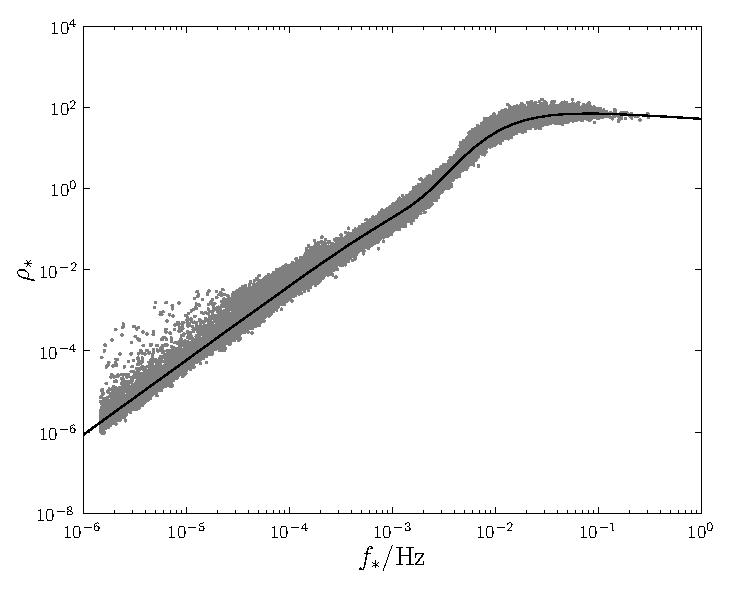
\includegraphics[width=0.6\textwidth]{./images/Fig_SNR_scaled_fit}
 \caption{Scaled signal-to-noise ratio for EMRBs as a function of characteristic frequency. The fitted curve from \eqnref{scaled-SNR} is indicated by the line.\label{fig:scaled-SNR}}%The reduced chi-squared value of the fit is $\chi^2/\nu = 4.4653$.
   \end{center}
\end{figure}
The curve shows that EMRB SNR does scale as expected, and $\rho_\ast$ can be described as a one-parameter curve. There remains some scatter about this (removing the averaging over intrinsic parameters increases this to about an order of magnitude); however, it is good enough for rough calculations.

We approximate the trend with a parametrized curve
\begin{equation}
\rho_\ast = \alpha_1 f_\ast^{\beta_1} \left[1 + \left(\alpha_2 f_\ast\right)^{\beta_2}\right]\left[1 + \left(\alpha_3 f_\ast\right)^{\beta_3}\right]^{-\beta_4}.
\label{eq:scaled-SNR}
\end{equation}
To fit this, we treat the problem as if it were a likelihood maximisation, with each averaged point having a Gaussian likelihood with standard deviation defined from the scatter because of the variation in the intrinsic parameters. The optimised values for LISA are
\begin{equation}
\begin{split}
&\alpha_1 \simeq 8.93 \times 10^4; \ \  \alpha_2 \simeq 4.68 \times 10^2; \ \  \alpha_3 \simeq 1.84 \times 10^2;\\
&\beta_1 \simeq 1.84; \ \  \beta_2 \simeq 3.23; \ \  \beta_3 \simeq 1.27; \ \  \beta_4 \simeq 4.13.
\end{split}
\end{equation}

Using our fitted trends it is possible to invert \eqnref{SNR-scaling} to find the furthest distance that bursts from an MBH of a given mass are detectable. In calculating the maximum SNR it is necessary to decide upon a minimum periapse radius. For the optimal case with a maximally rotating MBH, the innermost periapsis is $r\sub{p} = r\sub{g}$. For a non-rotating MBH, the innermost periapsis would be $r\sub{p} = 4r\sub{g}$. \Figref{detect} shows the detectability limit for $\mu = 1 M_\odot$ and $\mu = 10 M_\odot$ COs.
\begin{figure}[!htp]
\begin{center}
 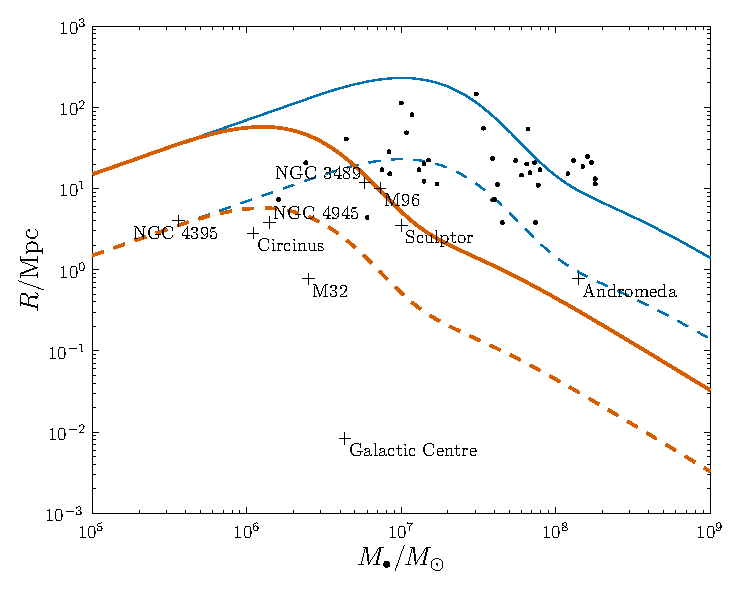
\includegraphics[width=0.6\textwidth]{./images/Fig_M_R_detect_1}
 \caption{Limit of detection for EMRBs originating from MBHs of mass $M_\bullet$ and distance $R$ with CO of mass $\mu = 1 M_\odot$ (dashed line) or $\mu = 10 M_\odot$ (solid line). The detection threshold is assumed to be $\rho = 10$. The thicker line is the limit for non-rotating MBHs, the thinner is for maximally rotating MBHs. Sources below the relevant line are potentially detectable. The trends should not be extrapolated to lower MBH masses.\label{fig:detect}}
   \end{center}
\end{figure}
The more massive COs are detectable to a greater distance, but are also the more likely sources since mass segregation ensures they are more likely to be on orbits that pass close to the MBH. Limits using periapsis of $r\sub{g}$ and $4r\sub{g}$ are shown: intermediate spin values would have limits between these two. In any case, these are strict bounds; it is unlikely that we would observe a burst from the optimal orbit. Therefore, bursts from MBHs outside the curve are impossible to detect and those inside may be possible, but need not be probable, to detect.

It appears that there are potentially many galaxies which could produce observable bursts. From our sample, all could be potentially detected. Andromeda could only be detected if it had a high spin value. It is therefore less promising than the others. NGC 3489, NGC 3368 and NGC 253 lie on the boundary of detectability for non-spinning sources with a $10 M_\odot$ CO. They are therefore of marginal interest: we do not necessarily need any special requirement for the spin, but such close orbits would be infrequent. NGC 4395, NGC 4945 and Circinus are around the boundary of detectability for a $1 M_\odot$ CO. Hence we could potentially see bursts from white dwarfs as well as BHs. M32 is the best extragalactic source, lying safely within the detection limit for $1 M\odot$ COs.

Examining M32 in detail, the trend between the periapse radius and SNR is shown in \figref{SNR-M32}.
\begin{figure}[!htp]
  \begin{center}
  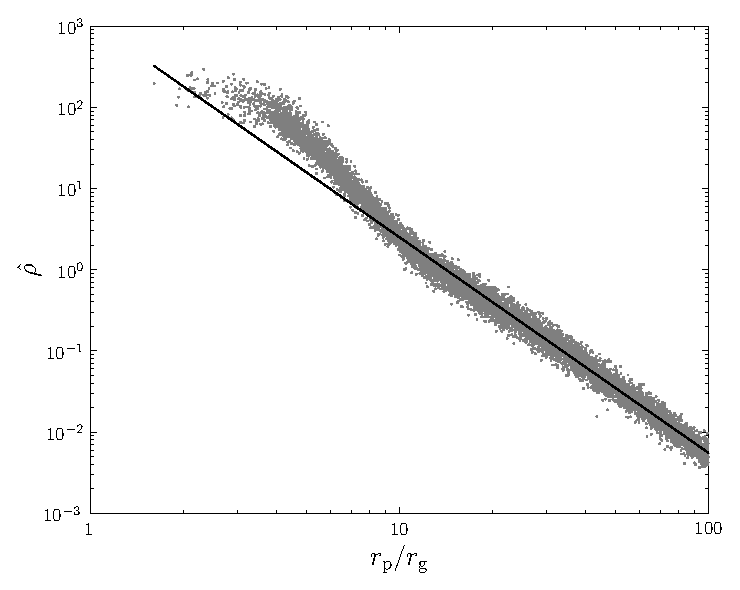
\includegraphics[width=0.6\textwidth]{./images/Fig_SNR_M32}
    \caption{Signal-to-noise ratio as a function of periapse radius for a $\mu = 1 M_\odot$ CO about the MBH of M32. The plotted points are the values obtained by averaging over each set of intrinsic parameters. The best fit line is $\log\left(\rho\right) = -2.65\log(r\sub{p}/r\sub{g}) + 3.05$. This is fitted to orbits with $r\sub{p} > 18.8 r\sub{g}$.\label{fig:SNR-M32}} % and has a reduced chi-squared value of $\chi^2/\nu = 1.26$
  \end{center}
\end{figure}
The fit is again for orbits with $f_\ast < 1 \times 10^{-3}\units{Hz}$ to avoid the bucket of the noise curve. Bursts for a $1 M_\odot$ ($10 M_\odot$) can be detected with $\rho > 10$ if the periapse is smaller than $7 r\sub{g}$ ($14 r\sub{g}$). We see that the general behaviour is the same as for the GC, but there are differences because of the position.

\subsection{Detection with eLISA}

We can repeat the analysis for eLISA. The scaled SNRs are shown in \figref{scaled-SNR-eLISA}.
\begin{figure}[!htp]
\begin{center}
 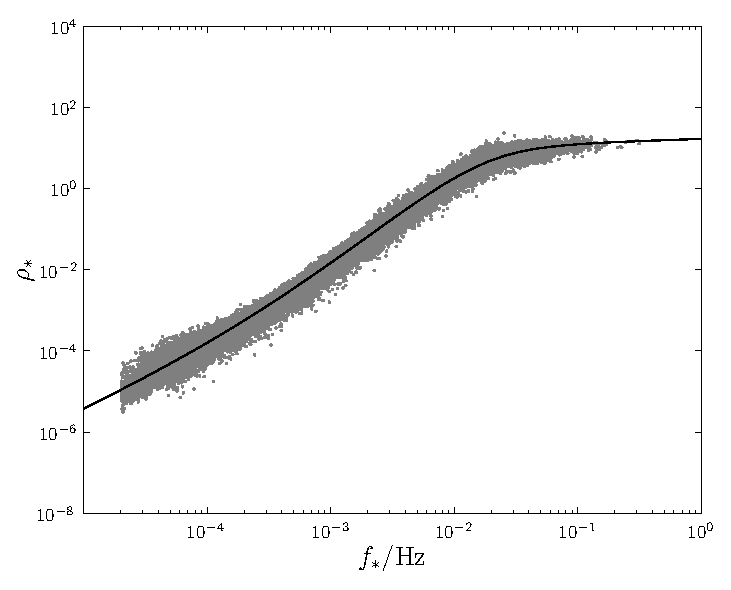
\includegraphics[width=0.6\textwidth]{./images/Fig_SNR_scaled_fit_eLISA}
 \caption{Scaled signal-to-noise ratio for EMRBs as a function of characteristic frequency for the eLISA design. The fitted curve from \eqnref{scaled-SNR} is indicated by the line.\label{fig:scaled-SNR-eLISA}}%The reduced chi-squared value of the fit is $\chi^2/\nu = 3.1063$.
   \end{center}
\end{figure}
Since Andromeda was only marginally of interest for the classic LISA design, we did not include it this time. The curve is fitted with
\begin{equation}
\begin{split}
&\alpha_1 \simeq 7.39 \times 10; \ \  \alpha_2 \simeq 4.99 \times 10^3; \ \  \alpha_3 \simeq 5.27 \times 10;\\
&\beta_1 \simeq 1.47; \ \  \beta_2 \simeq 0.85; \ \  \beta_3 \simeq 1.76; \ \  \beta_4 \simeq 1.25.
\end{split}
\end{equation}
Using this to find the detectability range results in the curves shown in \figref{detect-eLISA}.
\begin{figure}[!htp]
\begin{center}
 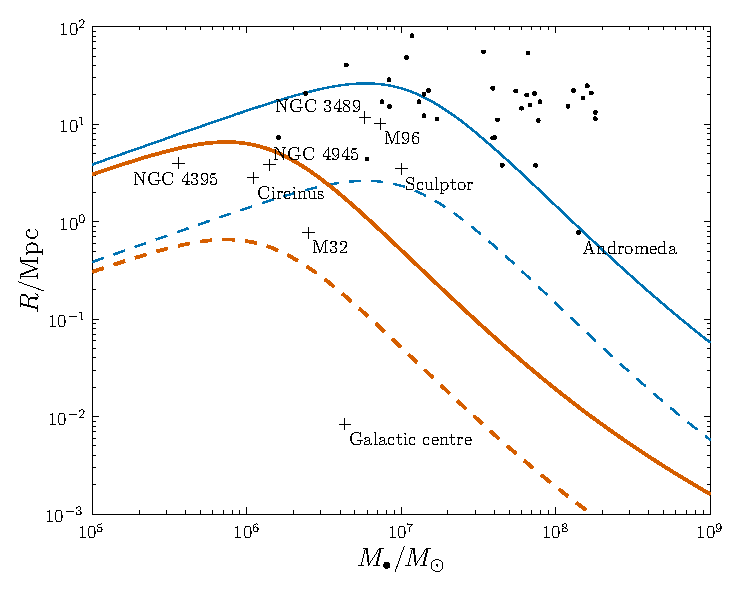
\includegraphics[width=0.6\textwidth]{./images/Fig_M_R_detect_2}
 \caption{Limit of detection using eLISA for EMRBs originating from MBHs of mass $M_\bullet$ and distance $R$ with CO of mass $\mu = 1 M_\odot$ (dashed line) or $\mu = 10 M_\odot$ (solid line). The detection threshold is assumed to be $\rho = 10$. The thicker line is the limit for non-rotating MBHs, the thinner is for maximally rotating MBHs. Sources below the relevant line are potentially detectable. The trends should not be extrapolated to lower MBH masses.\label{fig:detect-eLISA}}
   \end{center}
\end{figure}
The maximum distances are reduced compared to the LISA case, indicating that detectable bursts would be much rarer. There still remain a number of potential candidate galaxies. From our sample, Andromeda is on the very edge of possibility. NGC 3489, NGC 3368 and NGC 253 require a high spin, making them unlikely sources. Of the extragalactic sources, only M32 remains detectable with a $1 M_\odot$, and still it requires a non-zero spin.

Using either noise curve we see that EMRBs could potentially be seen from a range of galaxies. The Galaxy's MBH remains securely detectable in either case. M32 is the next best. MBHs with masses $\sim 10^6$--$10^7 M_\odot$ are observable to the greatest distance. We currently know of few MBHs with masses at the lower end of the spectrum ($10^5$--$10^6 M_\odot$) but these would be good potential candidates.